\subsubsection{\stid{3.13}CLOVER Sub-project SLATE}\label{subsubsect:slate}

\paragraph{Overview}

The Software for Linear Algebra Targeting Exascale (SLATE)
provides fundamental dense linear algebra capabilities
to DOE and the HPC community at large.
To this end, SLATE provides
parallel Basic Linear Algebra Subprograms (BLAS), norms,
linear systems solvers, least square solvers,
singular value and eigenvalue solvers.

The ultimate objective of SLATE is to replace the
venerable Scalable Linear Algebra PACKage (ScaLAPACK) library,
which has become the industry standard for dense linear algebra operations
in distributed-memory environments.
After two decades of operation,
ScaLAPACK is past the end of its life cycle and overdue for a replacement,
as it can hardly be retrofitted to support GPUs,
which are an integral part of today's HPC hardware infrastructure.

Primarily, SLATE aims to extract the full performance potential and maximum
scalability from modern HPC machines with large numbers nodes,
large numbers of cores per node, and multiple GPUs per node.
For typical dense linear algebra workloads, this means getting close
to the theoretical roofline peak performance and scaling to the full size of
the machine.
This is accomplished in a portable manner by relying on standards
like MPI and OpenMP.

SLATE functionalities will first be delivered to the ECP applications
that most urgently require SLATE capabilities
(NWChem, GAMESS, EXAALT, QMCPACK, CANDLE, etc.)
and to other software libraries
that rely on underlying dense linear algebra services
(STRUMPACK, SuperLU, etc.).
Figure~\ref{fig:slate-architecture} shows the role of SLATE
in the ECP software stack.

While the initial objective of SLATE is to serve as a successful,
drop-in replacement for ScaLAPACK with support for GPU accelerators,
the ultimate goal of SLATE is to deliver dense linear algebra capabilities
beyond the capabilities of ScaLAPACK.
This includes new features such as communication-avoiding
algorithms and randomization algorithms, as well as the potential to
support variable size tiles and block low-rank compressed tiles.

\begin{figure}[htb]
    \centering
    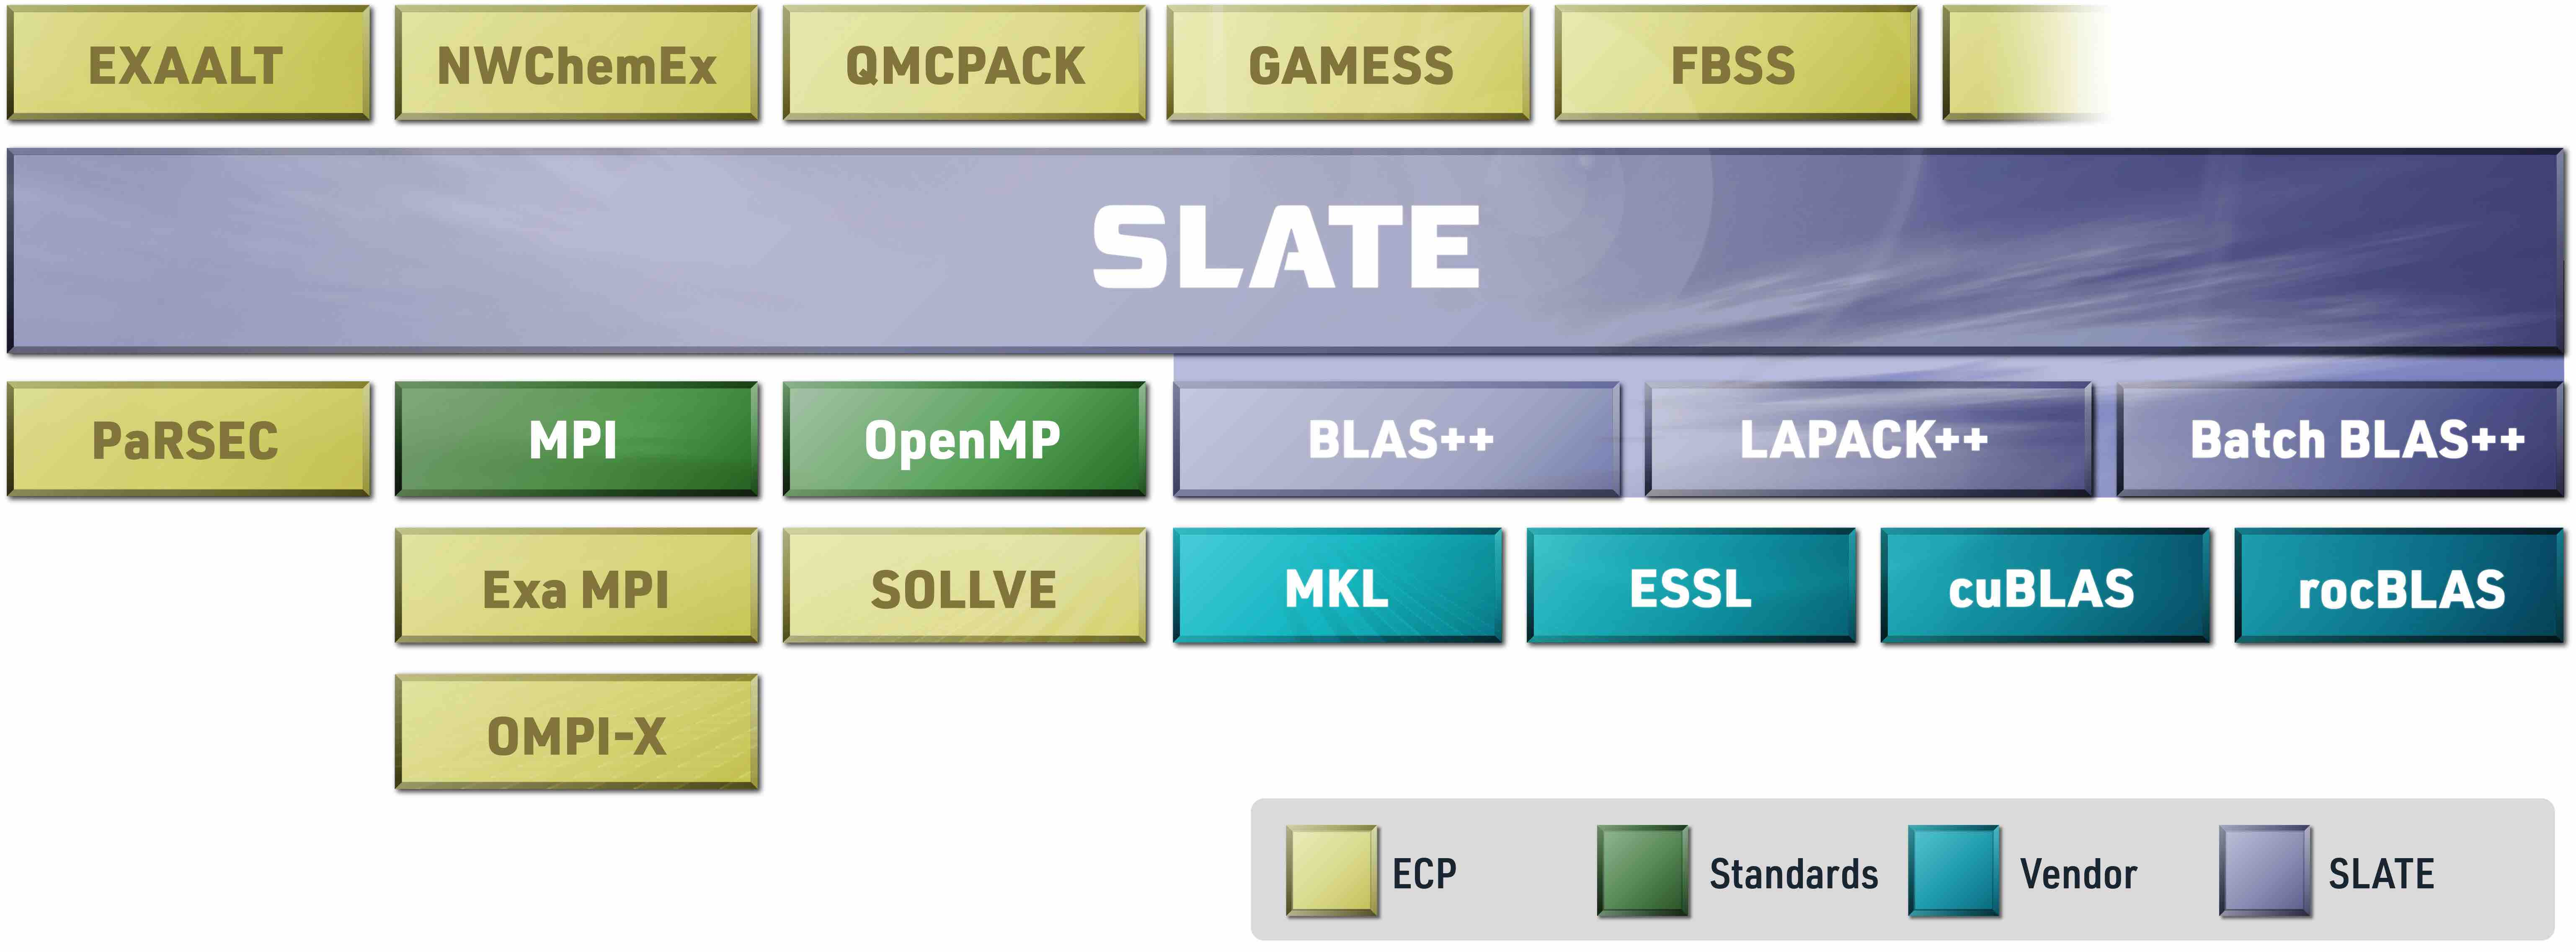
\includegraphics[width=0.75\textwidth]{projects/2.3.3-MathLibs/2.3.3.13-CLOVER/SLATE-architecture.jpg}
    \caption{\label{fig:slate-architecture}
    SLATE in the ECP software stack.}
\end{figure}

\paragraph{Key  Challenges}

\begin{enumerate}

\item
\textbf{Designing from the ground up:}
The SLATE project's primary challenge stems from the need to design the package
from the ground up, as no existing software package offers
a viable path forward for efficient support of GPUs
in a distributed-memory environment.

\item
\textbf{Facing harsh hardware realities:}
SLATE is being developed in a difficult hardware environment, where virtually
all the processing power is on the GPU side.
Achieving efficiency requires aggressive offload to GPU accelerators
and careful optimization of multiple bottlenecks, including 
interconnect technology lagging behind the computing
capabilities of the GPUs.

\item
\textbf{Facing harsh software realities:}
SLATE is being developed using cutting-edge software technologies,
and relies on modern C++ features and recent extensions
to the OpenMP standard, many of which are not fully supported by compilers
and their runtime environments.
In terms of GPU acceleration, standardized solutions are still in flux.
Also, while complete parallel programming frameworks exist, at this stage
they have to be considered research prototypes.

\end{enumerate}

\paragraph{Solution Strategy}

\begin{enumerate}

\item
\textbf{Evolving design:}
Due to the inherent challenges of designing a software package
from the ground up, the SLATE project started
with a careful analysis of the existing and emerging
implementation technologies~\cite{abdelfattah2017roadmap},
and followed with a phase
of laying out the initial design~\cite{kurzak2017designing}.
Since then, the team rolls out new computational routines every quarter.
While we continue to refactor as needed to achieve high performance, the basic
design has solidified and been published~\cite{gates2019slate-design}.

\item
\textbf{Focus on GPUs:}
Efficient GPU acceleration is the primary focus of performance
engineering efforts in SLATE.
Where applicable, highly optimized vendor implementations of GPU operations
are used, such as the batched \texttt{gemm} routine.
Where necessary, custom GPU kernels are developed, as in the case of computing
matrix norms.
Care is taken to hide communication by overlapping it with GPU computations.

\item
\textbf{Community engagement:}
The SLATE team interacts on a regular basis with the OpenMP community,
represented in ECP by the SOLLVE project, and with the MPI community,
represented in ECP by the OMPI-X project and the Exascale MPI project.
The SLATE team also engages the vendor community through our contacts
at Cray, IBM, Intel, NVIDIA, AMD, and ARM.

\end{enumerate}

\paragraph{Recent Progress}

% During 2018, the SLATE team implemented parallel BLAS, parallel norms,
% linear system solvers (LU, Cholesky, Hermitian indefinite $LTL^T$),
% and least squares solvers (QR, LQ).
During 2019, the SLATE team continued to add to its suite:
mixed-precision linear solvers for LU and Cholesky in March,
matrix inversion for LU and Cholesky in June,
and Hermitian eigenvalue and singular value solvers in September.
Routines are available in the four standard precisions (single, double,
complex-single, complex-double).
% We also continued to implement performance improvements, such as a CPU--GPU
% coherency protocol inspired by the MOSI cache consistency protocol, and
% improved handling of row-major matrices for efficient row-swapping in LU.
In addition to SLATE's native C++ API, compatibility APIs for LAPACK
and ScaLAPACK users are also provided, so that SLATE can serve
as a drop-in replacement.
All developments are documented in SLATE Working Notes
\footnote{\url{http://www.icl.utk.edu/publications/series/swans}.}


\paragraph{Next Steps}

\begin{enumerate}

\item
\textbf{Users' Guide and Developers' Guide:}
These guides will supplement SLATE's online Doxygen documentation by thoroughly
explaining both SLATE's public interface---how to integrate it into an
application, with examples---as well as SLATE's internal design, to help
new developers and outside collaborators understand the codebase. As living
documents, they will be continually updated as SLATE matures.

\item
\textbf{Band solvers:}
To SLATE's existing general band LU solvers,
we are adding Hermitian band Cholesky factorization and solve,
along with Hermitian band BLAS and norm routines.

\item
\textbf{Performance improvements:}
We have observed several routines that are not performing as well as expected.
In some cases, such as in QR, LQ, and parallel norms, we have already identified
improvements to be made to the algorithm, such as refactoring loops to improve
parallelism. In other cases, we are analyzing traces to identify and
correct problems.

\item
\textbf{Generalized Hermitian eigenvalue solver:}
We will extend SLATE's Hermitian eigenvalue solver to
handle generalized Hermitian-definite eigenvalue problems, of the form
$Ax = \lambda Bx$, $ABx = \lambda x$, or $BAx = \lambda x$.
These are of strong interest in mechanics and chemistry applications,
among others.

\item
\textbf{New C++, C, and Fortran application programming interfaces (APIs):}
The BLAS and (Sca)LAPACK APIs have served well over the past 40 years, but are
rooted in out-dated FORTRAN 77 limitations such as cryptic 5--6 letter
abbreviations (e.g., \texttt{dgemm, dgesv}). For SLATE, we will design a new,
user-friendly C++ interface (e.g., \texttt{multiply, solve}, respectively). New
C and Fortran APIs will also give better direct access to SLATE's features and
Matrix objects, without requiring use of our ScaLAPACK compatibility interface.

\item
\textbf{Non-symmetric eigenvalue problem:}
Computing the non-symmetric eigenvalue problem is significantly more
computationally expensive than the Hermitian eigenvalue problem. Our
implementation will leverage the latest advances, such as aggressive early
deflation, to achieve high performance.

\end{enumerate}
